\appendix

\chapter{Aufgabenstellung}
\label{AnhangAufgabenstellung}

Die Aufgabenstellung wurde im Februar 2018 übergeben und beinhaltet neben der Erläuterung der Aufgabe, weitere Anforderungen und Termine.

Dieses Dokument ist auch im digitalen Anhang \ref{AnhangDig} einsehbar.

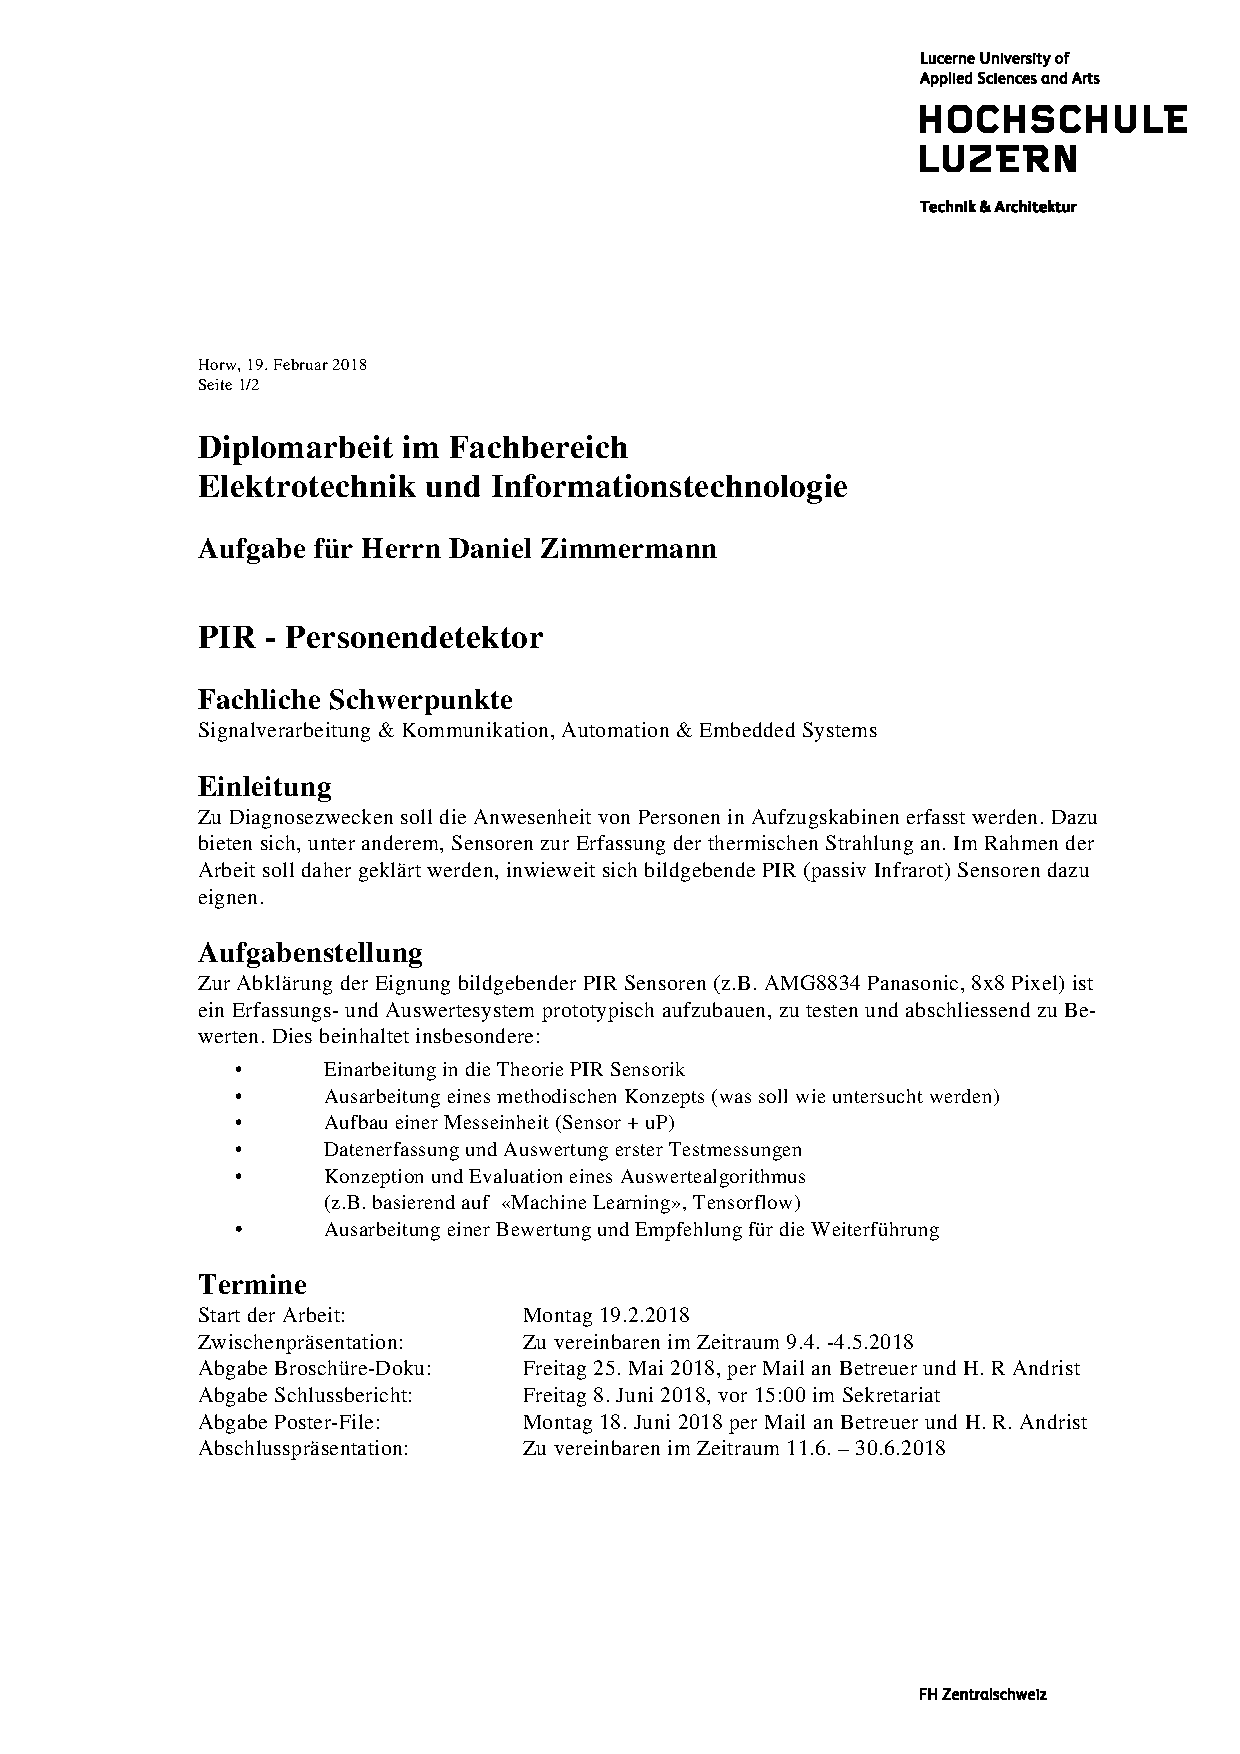
\includepdf[pages=-]{Anhang/Aufgabenstellung.pdf}

\chapter{Meilensteinplan}
Der Meilensteinplan wurde in der Initialisierungsphase erstellt und während dem Projektablauf angepasst. Die Meilensteine wurden farblich unterteilt. Die Unterteilungen sind in der Legende beschrieben. 

Dieses Dokument ist auch im digitalen Anhang \ref{AnhangDig} einsehbar.

\label{AnhangA}
\includepdf[pages=1,angle=90]{Anhang/Meilensteinplan_BAT_P1_V3.pdf}

\chapter{Detaillierter Projektplan}
\label{AnhangB}

Der detaillierte Projektplan gibt alle wesentlichen Tätigkeiten während des gesamten Projekt wieder. Dabei sind die Projektabschnitte und die Meilensteine angegeben.

Der Projektplan wurde für eine bessere Übersicht in zwei Teile unterteilt. 
\begin{itemize}
\item Der erste Teil ist der Zeitraum von der Initialisierung bis zur Zwischenpräsentation.

\item Der zweite Teil ist der Zeitraum von der Zwischenpräsentation bis zur Projektbeendigung.

\end{itemize}

Die einzelnen Tätigkeiten wurden auf zeitliche Aufwendungen geschätzt und der effektive Aufwand wird als Soll-Ist-Vergleich angegeben. 
Jedem Projektabschnitt werden die Zeitaufwendungen separat angerechnet. In jedem Teil ist in \textcolor{yellow}{gelber} Markierung die gesamthafte zeitliche Aufwendung angegeben.


Dieses Dokument ist auch im digitalen Anhang \ref{AnhangDig} einsehbar.


%\includepdf[pages=1,angle=90]{Anhang/01_Detaillierter Projektplan BAT V3.pdf}

%\includepdf[pages=1,angle=90]{Anhang/02_Detaillierter Projektplan BAT V3.pdf}



\chapter{Risikomanagement}
\label{AnhangC}
\setcounter{page}{9}
Das Risikomanagement wurde in der Initialisierungsphase erstellt und gibt Auskunft, welche Risiken bei dieser Arbeit zu beachten sind.

Eine Bewertung der Wahrscheinlichkeiten und den Auswirkungen gibt Auskunft, welche Risiken vorrangig beachtet werden müssen.  Dabei wurden diese in Standardrisiken und Projektbezogene Risiken unterteilt.

Dieses Dokument ist auch im digitalen Anhang \ref{AnhangDig} einsehbar.

\includepdf[pages=-,angle=90]{Anhang/Risikomanagement_V2.pdf}
\chapter{Übersicht Aufzugsprofile }
\label{AnhangD}

Es werden nachfolgend die drei verschiedenen Aufzugsprofile abgebildet. Dabei werden die wichtigsten Eigenschaften der erstellten Profile dargelegt. Daneben werde die Messpositionen, der verschiedenen Personenmessung mit den Buchstaben aus Unterkapitel \ref{subsec:Personen} angegeben. Die Buchstaben K, M und G stehen für die Probandengrössen; klein, mittel und gross, welche auch in  Unterkapitel \ref{subsec:Personena} erläutert sind.
\newpage


\section{Profil 1}
Beim Profil 1 handelt es sich um einem mittelgrossen Aufzug. Die Messungen wurde am 28.03.2018 am Messort Stansstad Bahnhofstrasse erstellt. Das Alter des Aufzugs mit der Kommissionsnummer 11018490 ist vom Baujahr 2017.
 


		\begin{figure}[!ht]
	\centering
	\begin{minipage}[b]{0.3\linewidth}
		\centering
		\includegraphics[width=0.9\linewidth]{fig/Gesamt1.jpeg}
		\caption{Gesamtbild}
		\label{fig:profilAnhang1}
	\end{minipage}
	\begin{minipage}[b]{0.3\linewidth}
		\centering
		\includegraphics[angle=270, width=0.9\linewidth]{fig/Raster1.jpg}
		\caption{Messraster}
		\label{fig:profilAnhang2}
	\end{minipage}
	\begin{minipage}[b]{0.3\linewidth}
		\centering
		\includegraphics[width=0.9\linewidth]{fig/beleuchtung1.jpeg}
		\caption{Beleuchtung}
		\label{fig:profilAnhang3}
	\end{minipage}
\end{figure}

\begin{table}[H]
	\centering
	\caption{Aufzugseigenschaften Profil 1}
	\label{aufzug1}
	\begin{tabular}{|c|c|c|c|c|c|}
		\hline
		\rowcolor[HTML]{9B9B9B} 
		\cellcolor[HTML]{9B9B9B}{\color[HTML]{333333} }                                                                                             & {\color[HTML]{333333} \textbf{Breite {[}m{]}}} & {\color[HTML]{333333} \textbf{Höhe {[}m{]}}} & {\color[HTML]{333333} \textbf{Tiefe {[}m{]}}} & \textbf{Bodenfäche  {[}$m^2${]}} & \textbf{Auslegung  } \\ \cline{2-6} 
		\multirow{-2}{*}{\cellcolor[HTML]{9B9B9B}{\color[HTML]{333333} \textbf{\begin{tabular}[c]{@{}c@{}}Aufzugs-\\ eigenschaften\end{tabular}}}} & 1.401                                          & 2.127                                        & 1.105                                         & 1.548                            & 8 Pers.                \\ \hline
		\rowcolor[HTML]{9B9B9B} 
		\cellcolor[HTML]{9B9B9B}                                                                                                                    & \textbf{Decke}                                 & \textbf{Boden}                               & \textbf{Front}                                & \textbf{Seitenwände}             & \textbf{Beleuchtung}       \\ \cline{2-6} 
		\multirow{-2}{*}{\cellcolor[HTML]{9B9B9B}\textbf{Materialaufbau}}                                                                           & Edelstahl                                      & Gummi                                        & Edelstahl                                     & Laminat                          & LED Strips                 \\ \hline
	\end{tabular}
\end{table}

\begin{table}[H]
	\centering
	\caption{Temperaturwerte Profil 1}
	\label{temp1}
	\begin{tabular}{|c|c|c|c|}
		\hline
		\rowcolor[HTML]{9B9B9B} 
		\cellcolor[HTML]{9B9B9B}{\color[HTML]{333333} }                                                                                                   & {\color[HTML]{333333} \textbf{Aussentemp. Aufzug}} & {\color[HTML]{333333} \textbf{Innentemp. Aufzug}} & {\color[HTML]{333333} \textbf{Oberflächentemp.}} \\ \cline{2-4} 
		\multirow{-2}{*}{\cellcolor[HTML]{9B9B9B}{\color[HTML]{333333} \textbf{\begin{tabular}[c]{@{}c@{}}Temperatur\\ Messdaten in °C\end{tabular}}}} & 19.9                                               & 20.1                                              & 16.5                                             \\ \hline
	\end{tabular}
\end{table}

 \textbf{Messpositionen:}\\
\textbf{1. Person Kat. K:} A, B, D, E, G, I, J\\
\textbf{1. Person Kat. G:} A, B, D, E, G, I, J\\
\textbf{2. Person Kat. K,G:} AB, AC, AI, DE, DF, GC, JE, JI  \\
\textbf{2. Person Kat. M,G:} AB, AC, AI, DE, DF, GC, JE, JI  \\
\textbf{3. Person Kat. K,M,G:} AEI, ABC, IEA, GEI, GKI, HDI, JHL \\
\textbf{4. Person Kat, K,K,M,G:} ACDF, CAFD, ACJL, ADGJ, DFGI, GJCF \\
\textbf{Trainingsetgrösse:}         151936 Frames \\
	
	\newpage
	
	
	\section{Profil 2}
Beim Profil 2 handelt es sich um einen grossen Aufzug. Die Messungen wurde am 10.05.2018 am Messort Wolfenschiessen Hauptstrasse erstellt. Das Alter des Aufzugs mit der Kommissionsnummer 20052781 ist vom Baujahr 2018.

	
	
		\begin{figure}[!ht]
	\centering
	\begin{minipage}[b]{0.3\linewidth}
		\centering
		\includegraphics[angle=270, width=0.9\linewidth]{fig/Gesamt2.jpg}
		\caption{Gesamtbild}
		\label{fig:profilAnhang4}
	\end{minipage}
	\begin{minipage}[b]{0.3\linewidth}
		\centering
		\includegraphics[angle=270,width=0.9\linewidth]{fig/Raster2.jpg}
		\caption{Messraster}
		\label{fig:profilAnhang5}
	\end{minipage}
	\begin{minipage}[b]{0.3\linewidth}
		\centering
		\includegraphics[angle=180,width=0.9\linewidth]{fig/beleuchtung2.jpg}
		\caption{Beleuchtung}
		\label{fig:profilAnhang6}
	\end{minipage}
\end{figure}

\begin{table}[H]
	\centering
	\caption{Aufzugseigenschaften Profil 2}
	\label{aufzug2}
	\begin{tabular}{|c|c|c|c|c|c|}
		\hline
		\rowcolor[HTML]{9B9B9B} 
		\cellcolor[HTML]{9B9B9B}{\color[HTML]{333333} }                                                                                             & {\color[HTML]{333333} \textbf{Breite {[}m{]}}} & {\color[HTML]{333333} \textbf{Höhe {[}m{]}}} & {\color[HTML]{333333} \textbf{Tiefe {[}m{]}}} & \textbf{Bodenfäche  {[}$m^2${]}} & \textbf{Auslegung  } \\ \cline{2-6} 
		\multirow{-2}{*}{\cellcolor[HTML]{9B9B9B}{\color[HTML]{333333} \textbf{\begin{tabular}[c]{@{}c@{}}Aufzugs-\\ eigenschaften\end{tabular}}}} & 1.401                                          & 1.105                                        & 2.127                                         & 1.548                            & 20 Pers.                \\ \hline
		\rowcolor[HTML]{9B9B9B} 
		\cellcolor[HTML]{9B9B9B}                                                                                                                    & \textbf{Decke}                                 & \textbf{Boden}                               & \textbf{Front}                                & \textbf{Seitenwände}             & \textbf{Beleuchtung}       \\ \cline{2-6} 
		\multirow{-2}{*}{\cellcolor[HTML]{9B9B9B}\textbf{Materialaufbau}}                                                                           & Edelstahl                                      & Granit                                        & Edelstahl                                     & Edelstahl                          & LED Spots                 \\ \hline
	\end{tabular}
\end{table}

\begin{table}[H]
	\centering
	\caption{Temperaturwerte Profil 2}
	\label{temp2}
	\begin{tabular}{|c|c|c|c|}
		\hline
		\rowcolor[HTML]{9B9B9B} 
		\cellcolor[HTML]{9B9B9B}{\color[HTML]{333333} }                                                                                                   & {\color[HTML]{333333} \textbf{Aussentemp. Aufzug}} & {\color[HTML]{333333} \textbf{Innentemp. Aufzug}} & {\color[HTML]{333333} \textbf{Oberflächentemp.}} \\ \cline{2-4} 
		\multirow{-2}{*}{\cellcolor[HTML]{9B9B9B}{\color[HTML]{333333} \textbf{\begin{tabular}[c]{@{}c@{}}Temperatur\\ Messdaten in °C\end{tabular}}}} & 22.2                                               & 22.5                                              & 19.7                                             \\ \hline
	\end{tabular}
\end{table}

 \textbf{Messpositionen:}\\
\textbf{1. Person Kat. K:} A, B, D, E, G, I, J\\
\textbf{1. Person Kat. G:} A, B, D, E, G, I, J\\
\textbf{2. Person Kat. K,G:} AB, AC, AI, DE, DF, GC, JE, JI   \\
\textbf{2. Person Kat. K,M:} AB, AC, AI, DE, DF, GC, JE, JI   \\
\textbf{3. Person Kat. K,M,K:} AEI, ABC, IEA, GEI, GKI, HDI, JHL \\
\textbf{4. Person Kat, K,K,M,G:} ACDF, CAFD, ACJL, ADGJ, DFGI, GJCF \\
\textbf{Trainingssetgrösse:} 153181 Frames


	\newpage
\section{Profil 3}
Beim Profil 3 handelt es sich um einen kleine Aufzug. Die Messungen wurde am 12.05.2018 am Messort Stansstad Dorfstrasse erstellt. Das Alter des Aufzugs mit der Kommissionsnummer 54004012294 ist vom Baujahr 1988.

		
		\begin{figure}[!ht]
	\centering
	\begin{minipage}[b]{0.3\linewidth}
		\centering
		\includegraphics[angle=270,width=0.9\linewidth]{fig/Gesamt3.jpg}
		\caption{Gesamtbild}
		\label{fig:profilAnhang7}
	\end{minipage}
	\begin{minipage}[b]{0.3\linewidth}
		\centering
		\includegraphics[angle=270,width=0.9\linewidth]{fig/Raster3.jpg}
		\caption{Messraster}
		\label{fig:profilAnhang8}
	\end{minipage}
	\begin{minipage}[b]{0.3\linewidth}
		\centering
		\includegraphics[angle=180,width=0.9\linewidth]{fig/beleuchtung3.jpg}
		\caption{Beleuchtung}
		\label{fig:profilAnhang9}
	\end{minipage}
\end{figure}

\begin{table}[H]
	\centering
	\caption{Aufzugseigenschaften Profil 3}
	\label{aufzug1}
	\begin{tabular}{|c|c|c|c|c|c|}
		\hline
		\rowcolor[HTML]{9B9B9B} 
		\cellcolor[HTML]{9B9B9B}{\color[HTML]{333333} }                                                                                             & {\color[HTML]{333333} \textbf{Breite {[}m{]}}} & {\color[HTML]{333333} \textbf{Höhe {[}m{]}}} & {\color[HTML]{333333} \textbf{Tiefe {[}m{]}}} & \textbf{Bodenfäche  {[}$m^2${]}} & \textbf{Auslegung  } \\ \cline{2-6} 
		\multirow{-2}{*}{\cellcolor[HTML]{9B9B9B}{\color[HTML]{333333} \textbf{\begin{tabular}[c]{@{}c@{}}Aufzugs-\\ eigenschaften\end{tabular}}}} & 1.095                                          & 2.105                                        & 1.246                                         & 1.548                            & 6  Pers.)                \\ \hline
		\rowcolor[HTML]{9B9B9B} 
		\cellcolor[HTML]{9B9B9B}                                                                                                                    & \textbf{Decke}                                 & \textbf{Boden}                               & \textbf{Front}                                & \textbf{Seitenwände}             & \textbf{Beleuchtung}       \\ \cline{2-6} 
		\multirow{-2}{*}{\cellcolor[HTML]{9B9B9B}\textbf{Materialaufbau}}                                                                           & Edelstahl                                      & Granit                                       & Edelstahl                                     & Kunststoff                         & Leuchtstoff                 \\ \hline
	\end{tabular}
\end{table}

\begin{table}[H]
	\centering
	\caption{Temperaturwerte Profil 3}
	\label{temp3}
	\begin{tabular}{|c|c|c|c|}
		\hline
		\rowcolor[HTML]{9B9B9B} 
		\cellcolor[HTML]{9B9B9B}{\color[HTML]{333333} }                                                                                                   & {\color[HTML]{333333} \textbf{Aussentemp. Aufzug}} & {\color[HTML]{333333} \textbf{Innentemp. Aufzug}} & {\color[HTML]{333333} \textbf{Oberflächentemp.}} \\ \cline{2-4} 
		\multirow{-2}{*}{\cellcolor[HTML]{9B9B9B}{\color[HTML]{333333} \textbf{\begin{tabular}[c]{@{}c@{}}Temperatur\\ Messdaten in °C\end{tabular}}}} & 17.5                                               & 17.7                                              & 17.5                                             \\ \hline
	\end{tabular}
\end{table}

 \textbf{Messpositionen:}\\
\textbf{1. Person Kat. K:} A, B, D, E, G, I, J\\
\textbf{1. Person Kat. G:} A, B, D, E, G, I, J\\
\textbf{2. Person Kat. K,K:} AB, AC, AI, DE, DF, GC, JE, JI   \\
\textbf{2. Person Kat. K,G:} AB, AC, AI, DE, DF, GC, JE, JI   \\
\textbf{3. Person Kat. K,G,K:} AEI, ABC, DEF, ABI, DHL, GEI, GKI, HDC \\
\textbf{4. Person Kat K,K,M,G:} ACDF, ACJL, ADGI, DFAC, DFGI, GJCF \\
\textbf{Trainingsetgrösse:}         154461 Frames \\			
			
		\chapter{Emissionsgradtabelle}
			\label{AnhangE}
			
			Die Emissionsgrade von Materialien variieren, daher wurde zur Übersicht eine entsprechende Emissionsgradtabelle angefügt. Die Emissionsgradtabelle wurde aus der Literatur von \cite{Thermoformeln} entnommen.
			
			
			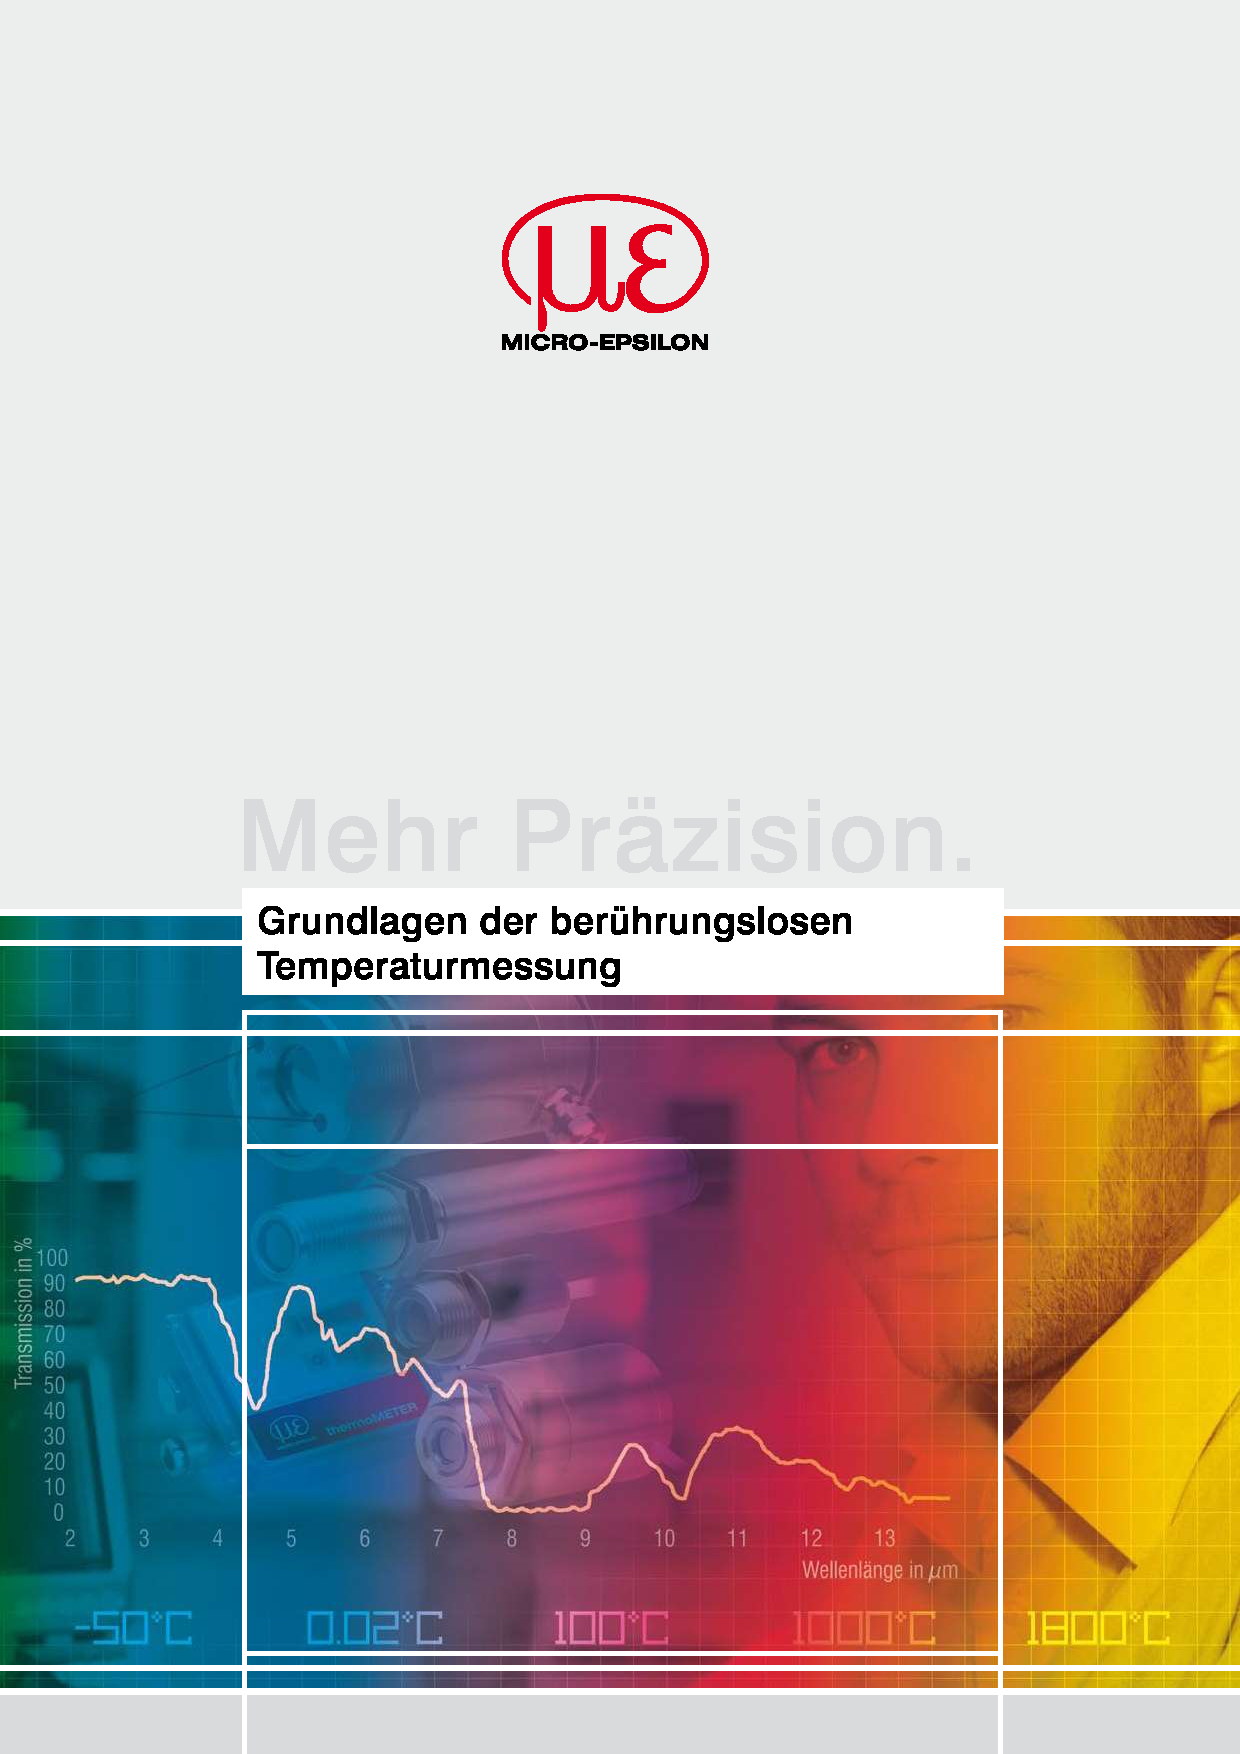
\includepdf[pages=-]{Anhang/emissionsgradtabelle.pdf}
			
			
			\chapter*{Digitale Projektanhänge}
			\label{AnhangDig}
			
			Der Projektanhang enthält neben dem Schlussbericht und dem Projektmanagement, alle Skizzen, Rohdaten in strukturierer Form. Alle Matlab und Python-Programme sind entsprechend kommentiert und geben Auskunft über die Funktionen. Jeder Unterordner enthält ein "readme", welches zusätzliche Informationen enthält..
			
			\section{Ordnerstruktur CD}
			
			
			Die beiliegende CD hat folgende Ordnerstruktur.
			
			\begin{enumerate}
				\item Abgabedokument
				\begin{itemize}
					\item BAT\_Schlussdokumentation
				\end{itemize}
				\item Projektmanagement
				\begin{itemize}
					\item Aufgabenstellung
					\item Meilensteinplan P2 V3
					\item Detaillierter Projektplan V3 Teil 1
					\item Detaillierter Projektplan V3 Teil 2
					\item Risikomanagement v3
					\item Besprechungsprotokolle
					\item Bestellungen
				\end{itemize}
				\item Testdurchführungen
				\begin{itemize}
					\item Testkonzepte \& Testmappen
					\item Matlab Messungen \& Skripts
				\end{itemize}
				\item Messdaten
				\begin{itemize}
					\item Testkonzepte \& Testmappen
					\item H-Term 
					\item ConvertValue\_V2
				\end{itemize}
				\item Software Personenerkennung
				\begin{itemize}
					\item 
					\item 
					\item 
					\item Datensätze
				\end{itemize}
				\item Profile
				\begin{itemize}
					\item Profile 1
					\item Profile 2
					\item Profile 3
					\item Testprofile 
					\item ConvertValue\_V2			
				\end{itemize}
				\item Datenblätter
				\begin{itemize}
					\item Panasonic AMG8834
					\item Melexis MLX90640
					\item Fluke TI-52-II
					\item Fluke TI 125 
				\end{itemize}
			\end{enumerate}
			
			\newpage
			

				
